\paragraph{Интегралы}~
\begin{enumerate}
\item $C\dot e = 0 \Rightarrow r = r_0 = const$
\item $(\v M_0, \v e_z) = 0, \quad \dot{\v e}_z = 0 \Rightarrow k_z = (\v k_O, \v e_z) = const $ \\
$k_z = (Ap \v e_\xi + Aq \v e_\eta + Cr \v e_\zeta, \sin \Theta \sin \varphi \cdot \v e_\xi + \sin \Theta \cos \varphi \v e_\eta - \cos \Theta \v e_\zeta = A\sin \Theta (p\sin \varphi + q \cos \varphi) + Cr_0 \cos \Theta = A \dot \psi \sin \Theta + C r_0 \cos \Theta = k = const$
\item $T + \Pi = h = const$\\
$\frac{1}{2}(ap^2 + Aq^2 + Cr^2 + mg l \cos \Theta = h$\\
$A(\dot \psi^2 \sin^2 \Theta + \dot \Theta^2) + Cr_0^2 + 2 mg l \cos \Theta = 2h$\\
$A(\dot \psi^2 \sin^2 \Theta + \dot \Theta^2) + 2mg l \cos \Theta = h^*, \quad h^* = 2h - Cr_0^2$\\
\end{enumerate}
Интегрирование: $2 \Rightarrow \dot \psi = \frac{k - Cr_0\cos \Theta}{A \sin^2 \Theta}$\\
\begin{flalign*}
& 3 \Rightarrow \frac{(k - Cr_0\cos \Theta)^2}{A\sin^2 \Theta} + A \dot \Theta^2 + 2m g l\cos \Theta = h^* &\\
& \dot \Theta^2 = f(\Theta), \quad f(\Theta) = \frac{1}{A}\left( h^* - rmg l \cos \Theta - \frac{(k - Cr_0\cos \Theta)^2}{A\sin^2 \Theta} \right) &\\
& \dot \Theta = \pm \sqrt{f(\Theta)} &\\
& \frac{d\Theta}{\sqrt{f(\Theta)}} = \pm dt &\\
& \int\limits_{\Theta_0}^\Theta \frac{d\xi}{\sqrt{f(\xi)}} = t - t_0 &\\
& \dot \Theta = \frac{kCr_0 \cos \Theta(t)}{A\sin^2 \Theta(t)} = f_1(t) &\\
& \psi = \int\limits_0^t f_1(\tau)d\tau = \psi(t) &\\
& \dot \varphi = r_0 - \dot \psi \cos \Theta = r_0 - \psi(t)\cos\Theta(t) = f_2(t) &\\
& \varphi = \int\limits_0^t f_2(\tau)d\tau &\\
\end{flalign*}

\subsubsection*{Геометрическая интерпретация}
\begin{flalign*}
& \cos \Theta = x &\\
& Ah^* - 2Amg l x - \frac{(Cr_0 x - k)^2}{1 - x^2} = A^2 f(\Theta) = A^2\dot \Theta^2 &\\
& F(x) = 2A m g l x + \frac{(Cr_0 x - k)^2}{1 - x^2} \leqslant Ah^* &\\
& F(x) = 2A m g l x + \frac{C^2 r_0^2(x^2 - 1) + C^2r_0^2 + k^2 - 2Cr_0kx}{1 - x^2} = &\\
& = 2 A mg l x - C^2 r_0^2 + \frac{(Cr_0 - k)^2(1 + x) + (Cr_0 + k)^2(1 - x)}{2(1 - x^2)} = &\\
& = 2A mg l x - C^2r_0^2 + \frac{1}{2}\left( \frac{(Cr_0 - k)^2}{1 - x} + \frac{(Cr_0 + k)^2}{1 + x} \right) &\\
& F'_x(x) = 2Am g l + \frac{1}{2} \left( \frac{(Cr_0 - k)^2}{(1 - x)^2} - \frac{(Cr_0 + k)^2}{(1 + x)^2}\right) &\\
& F''_x(x) = 0 + \frac{(Cr_0 - k)^2}{(1 - x)^3} + \frac{(Cr_0 + k)^2}{(1 + x)^3} \geqslant 0, \quad \forall x \in (-1, 1) &\\
\end{flalign*}
\begin{figure}[H]
  \centering
  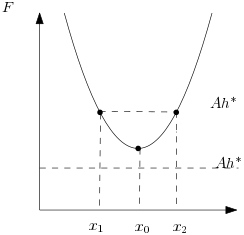
\includegraphics[width=5cm]{fig14.png} 
\end{figure}  
\begin{enumerate}
\item $h^* = \frac{F(x_0)}{A} \Rightarrow x = x_0,\;\; \Theta = \arccos x_0 = const$
\begin{figure}[H]
  \centering
  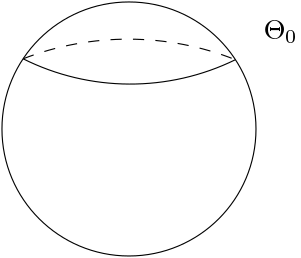
\includegraphics[width=4cm]{fig15.png} 
\end{figure}
\item $h^* > \frac{F(x_0)}{A}$: $\Theta_{min} = \arccos x_2$,~~ $\Theta_{max} = \arccos x_1$
\begin{figure}[h]
  \centering
  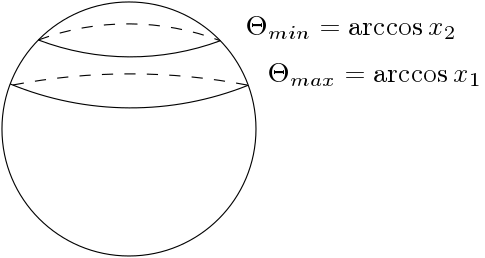
\includegraphics[width=6cm]{fig16.png} 
\end{figure}
\end{enumerate}

\begin{flalign*}
& \dot \psi = \frac{Cr_0x - k}{A(1 - x^2)} = 0 \Leftrightarrow x = x_* = \frac{k}{Cr_0} &\\
& F'_*(x_*) = 2Amgl > 0 &\\
\end{flalign*}

\begin{figure}[h]
  \centering
  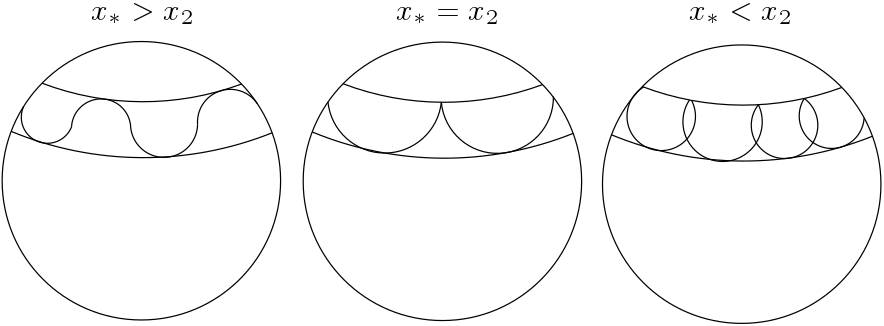
\includegraphics[width=14cm]{fig17.png} 
\end{figure}


\begin{ntc}
Если угловая скорость собственного вращения много больше скорости прецессии, т.е. $\dot \varphi \gg \dot \psi$, тело совершает псевдорегулярную пресессию.
\end{ntc}

\paragraph{Основные теоремы динамики}
\begin{flalign*}
& \v p = m \v v_s &\\
& \v k_O = [\v r_s, m \v v_s] + J_s \v \omega &\\
& T = \frac{1}{2}mv_s^2 + \frac{1}{2}(J_s\v \omega, \v \omega) &\\
\end{flalign*}

\begin{flalign*}
& \dot{\v p} = \sum\limits_{i = 1}^N F_i^{(e)}= \v F &\\
& \dot{\v k_O} = \sum p\v r_i, \v F_i^{(e)} = \v M_O &\\
& \dot T = \sum (\v F_i^{(e)}, \v v_i) &\\
\end{flalign*}

\begin{ntc}
\[
	\sum(\v F_i^{(e)}, \v v_i) = \dot T = (m \v w_s, \v v_s) + (\dot{(J_s\v\omega)}, \v \omega) = (\v F, \v v_s) + (\v M_s, \v \omega)
\]
\end{ntc}

\begin{ass}
Мощность внешних сил, действующих на твердое тело определяется равенством
\[
	\sum(\v F_i^{(e)}, \v v_i) = (\v p, \v v_p) + (\v M_p, \v \omega),
\]
где $p$ --- произвольная точка тела.
\end{ass}
\begin{proof}
\begin{flalign*}
& \sum (\v F_i^{(e)}, \v v_i) = \sum (\v F_i^{(e)}, \v v_p + [\v \omega, \rho_i]) = \left(\sum \v F_i^{(e)}, \v v_p\right) + (\v \omega, \sum [\v \rho_i, \v F_i]) = &\\
& = (\v p, \v v_p) + (\v M_p, \v \omega) &\\
\end{flalign*}
\end{proof}

\begin{df}
Две системы сил (в совокупности с точками их приложения), действующих на твердое тело называются эквивалентными, если они вызывают одно и то же движение тела.
\[
	\{ \v F_i, p_i \} \sim \{\v F_i', p_i'\}
\]
\end{df}
\begin{cor}
\[
	\{ \v F_i, p_i \} \sim {\v F_i', p_i'} \Leftrightarrow 
	\begin{cases}
	\sum \v F_i = \sum \v F_i' \\
	\sum [\v{OP}, \v F_i] = \sum [\v{OP}', \v F_i'] \\
	\end{cases}
\]	
\end{cor}
\begin{cor}
\[
	\{\v F_i, p_i\} \sim \{\v F, \v M_O, O\}, \quad \v F = \sum \v F_i,\;\; \v M_O = \sum [\v{OP}, \v F_i]
\]
\end{cor}
\begin{df}
$\v R$ --- равнодействующая системы сил $\{ \v F_i, \v p_i \}$, если существует точка $O$ тела, такая что $\{ \v F, p_i \} \sim \{\v R, O\}$
\end{df}
\begin{xmp}
Для двух сил, приложенных к разным концам твердого стержня в противоположном направлении, равнодействующая не существует.
\end{xmp}
\begin{xmp}
\[
	\{ m_i\v g, P_i \} \sim \{ m \v g, S \}
\]
\begin{flalign*}
& \sum m_i \v \rho = \left(\sum m_i\right)\v g = m\v g &\\
& \sum [\v {OP}, m_i \v g] = \sum [m_i \v {OP}, \v g] = \left[\sum m_i \v{OP}, \v g\right] = [m \v r_s, \v g] = [\v r_s, m\v g] &\\
\end{flalign*}
\end{xmp}

\[
	\v M_{O'} = \v M_O + [\v F, \v{OO'}]
\]

\begin{teo}
Если главный вектор внешних сил, действующих на твердое тело отличен от нуля, то существует такая точка, при приведении к которой, главный вектор и главный момент параллельны.
\[
	\v F \neq 0 \quad \exists A: \v M_A \parallel \v F
\]
\end{teo}
\begin{proof}
\begin{flalign*}
& \v M_a = \v M_O + [\v F, \v{OA}] = \lambda \v F \quad \big| \times \v F &\\
& [\v F, \v M_O] + \v F(\v F, \v{OA}) - F^2\v{OA} = 0 &\\
& \v{OA} = \frac{1}{F^2} [\v F, \v M_O] + \alpha \v F, \quad \forall \alpha = const
\end{flalign*}
\end{proof}
\begin{df}
Прямая, определяемая последним равенством называется осью динамического винта (осью минимальных моментов).
\end{df}
\begin{df}
$\lambda$ --- параметр винта.
\[
\lambda \v F = \v M_O + \left[ \v F, \frac{1}{F^2}[\v F, \v M_O] + \alpha \ F \right] = \v M_O + \frac{1}{F^2}\left( \v F(\v F, \v M_O) - F^2 \v M_O \right) = \frac{(\v F, \v M_O)}{F^2} \v F
\]
\[
	\lambda = \frac{(\v F, \v M_O)}{F^2}
\]
\begin{enumerate}
\item $\v F = 0: \quad \{ \v F_i, P_i\} \sim \{ \v M_O, O \}$
\item $\v F \neq 0, \lambda = 0: \{ \v F_i, P_i \} \sim \{\v R, A\}$
\item $\v F \neq 0, \lambda \neq 0: \{ \v F, P_i \} \sim \{\v F, \v M_A, A\}$
\end{enumerate}
\end{df}